\section*{Описание структур данных}

Для хранения строк, считанных из файла, используется массив указателей на строки (каждая строка имеет тип данных \textbf{char*}). Доступ к массиву осуществляется через указатель на него (тип \textbf{char**}). Память под строки и массив указателей на них выделяется динамически. Структура хранения данных указана на рис. \ref{data_schema}.

\begin{figure}[H]
	\centering
 	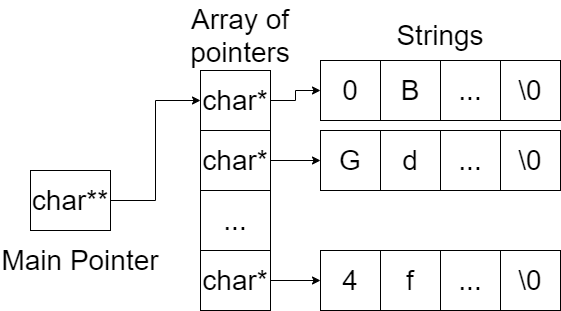
\includegraphics[width=0.6\linewidth]{photo/data_schema}
 	\caption{Структура хранения данных, считанных из файла}
 	\label{data_schema}
\end{figure}